\section{Chapter 4: Labor Market Equilibrium}

This chapter will study the notion of labor market equilibrium,
which is the outcome of the interaction between labor supply, labor demand,
and possibly external forces, such as government policies.


\begin{definition}[Invisible Hand Theorem] 
    
    If markets are competitive, and workers and 
    firms are free to enter and leave the market, then 
    the equilibrium allocation of workers and wages 
    will be efficient, in the sense that it maximizes 
    the total gains that workers and firms 
    obtain from trade with each other.

\end{definition}

%%%%%%%%%%%%%%%%%%%%%%%%%%%%%%%%%%%%%%%%%%%%%%%%%%%%%%%%%%%%%%%%%%%%%%%%%%%%%%%%%%%%%%%
%%%%%%%%%%%%%%%%%%%%%%%%%%%%%%%%%%%%%%%%%%%%%%%%%%%%%%%%%%%%%%%%%%%%%%%%%%%%%%%%%%%%%%%
\subsection{Equilibrium in a Single Labor Market}

\autoref{fig:ch_4p1_surplus}
illustrates a competitive labor market with an 
equilibrium at $(E^*, w^*)$.


\FloatBarrier

\begin{figure}[!htb]
    \centering
        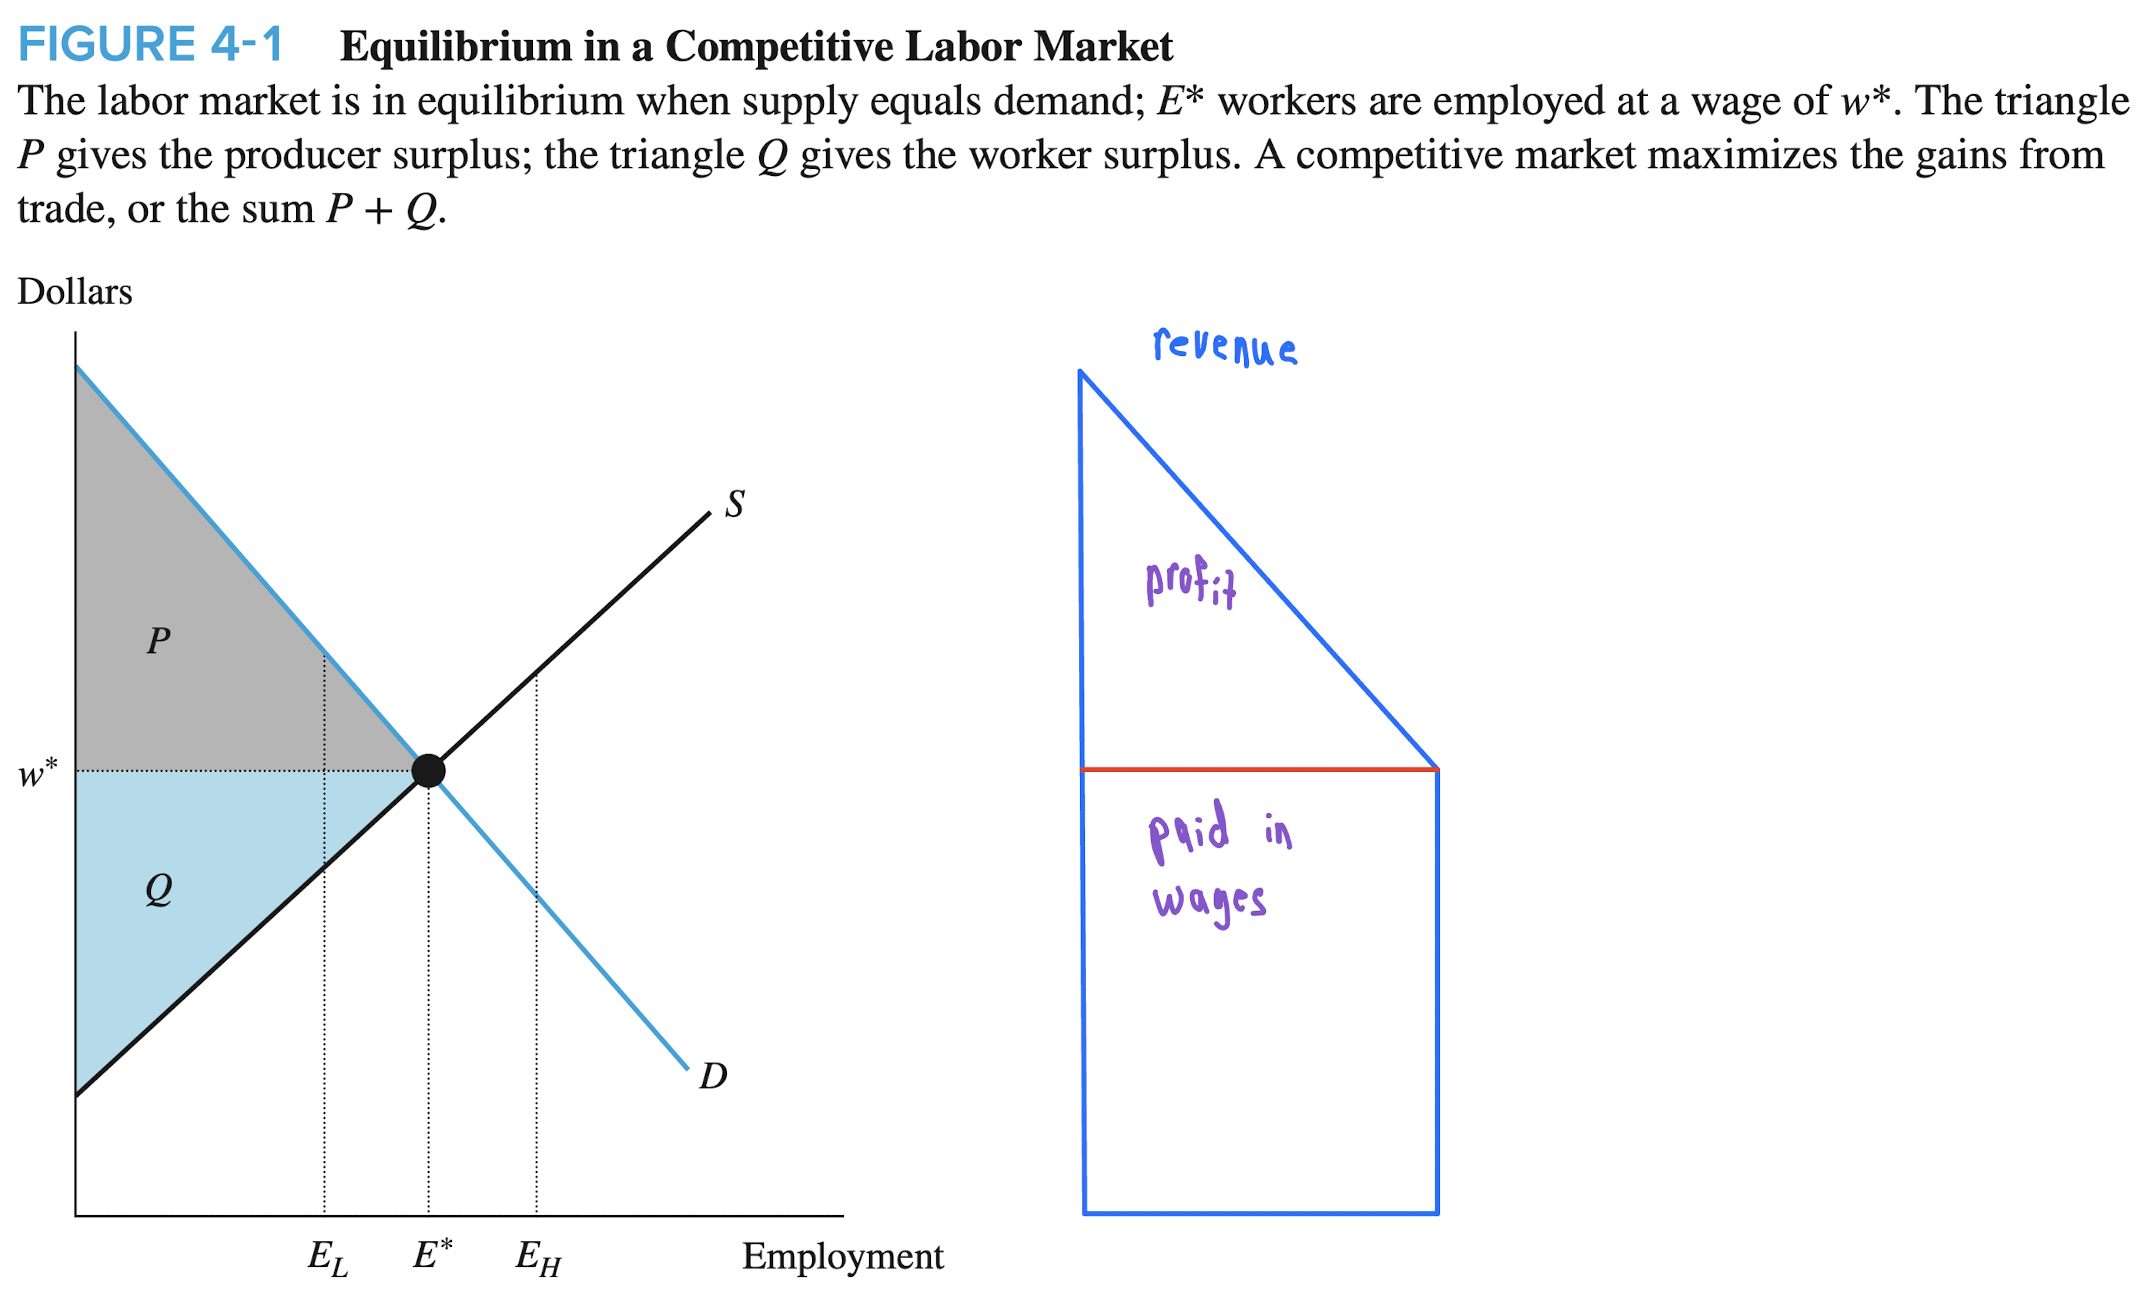
\includegraphics[width=0.95\textwidth]{../input/ch_4p1_surplus.png}
    \caption{Labor Market Surplus}
    \label{fig:ch_4p1_surplus}
\end{figure}

\FloatBarrier

Since the labor demand curve corresponds to the value of 
the marginal product, we can see that the area under the labor 
demand curve up to any given point corresponds to the total revenue
a firm receives from hiring that many workers.
Thus, since the equilibrium is at $(E^*, w^*)$, the
firm's total revenue is given by the area under the demand 
curve up to $E^*$, which is drawn out 
in blue in \autoref{fig:ch_4p1_surplus}.
Similarly, the area under the supply curve up to $E^*$,
their profit, or producer surplus (denoted $P$ in \autoref{fig:ch_4p1_surplus}), is 
given by the triangle above $w^*$ and below the labor 
demand curve.

\begin{definition}[Producer Surplus] 

    Producer surplus is the difference between the 
    revenue a firm receives and the cost it incurs.
    
\end{definition}

Similarly, workers are indifferent between working and not working 
along the labor supply curve. Thus, workers who are 
willing to work for less than $w^*$ (which is everyone 
except the final workers hired) receive a surplus.
This surplus is given by the triangle below $w^*$ and
above the labor supply curve, denoted $Q$ in 
\autoref{fig:ch_4p1_surplus}.

The gains from trade are given by the sum of the
producer and worker surplus: $P + Q$.
The competitive market equilibrium maximizes the 
gains from trade. Such an outcome that maximizes 
gains from trade is said to be ``efficient.''

\begin{questions}
    It's somewhat challenging for me to think about 
    how I should think about the connection between surplus 
    and wellbeing. I understood surplus as a clear quantitative 
    measure, but it seems like we would only care about it insofar as it 
    connects to something more like the wellbeing of the parties 
    involved. However, it's super unclear to me 
    if we're trying to connect it back to that 
    in any way.
\end{questions}

%%%%%%%%%%%%%%%%%%%%%%%%%%%%%%%%%%%%%%%%%%%%%%%%%%%%%%%%%%%%%%%%%%%%%%%%%%%%%%%%%%%%%%%
%%%%%%%%%%%%%%%%%%%%%%%%%%%%%%%%%%%%%%%%%%%%%%%%%%%%%%%%%%%%%%%%%%%%%%%%%%%%%%%%%%%%%%%
\subsection{Equilibrium across Labor Markets}

So far, we have focused on a single labor market.
Now, we turn to the case of multiple labor markets
linked by migration.


\begin{figure}[!htb]
    \centering
        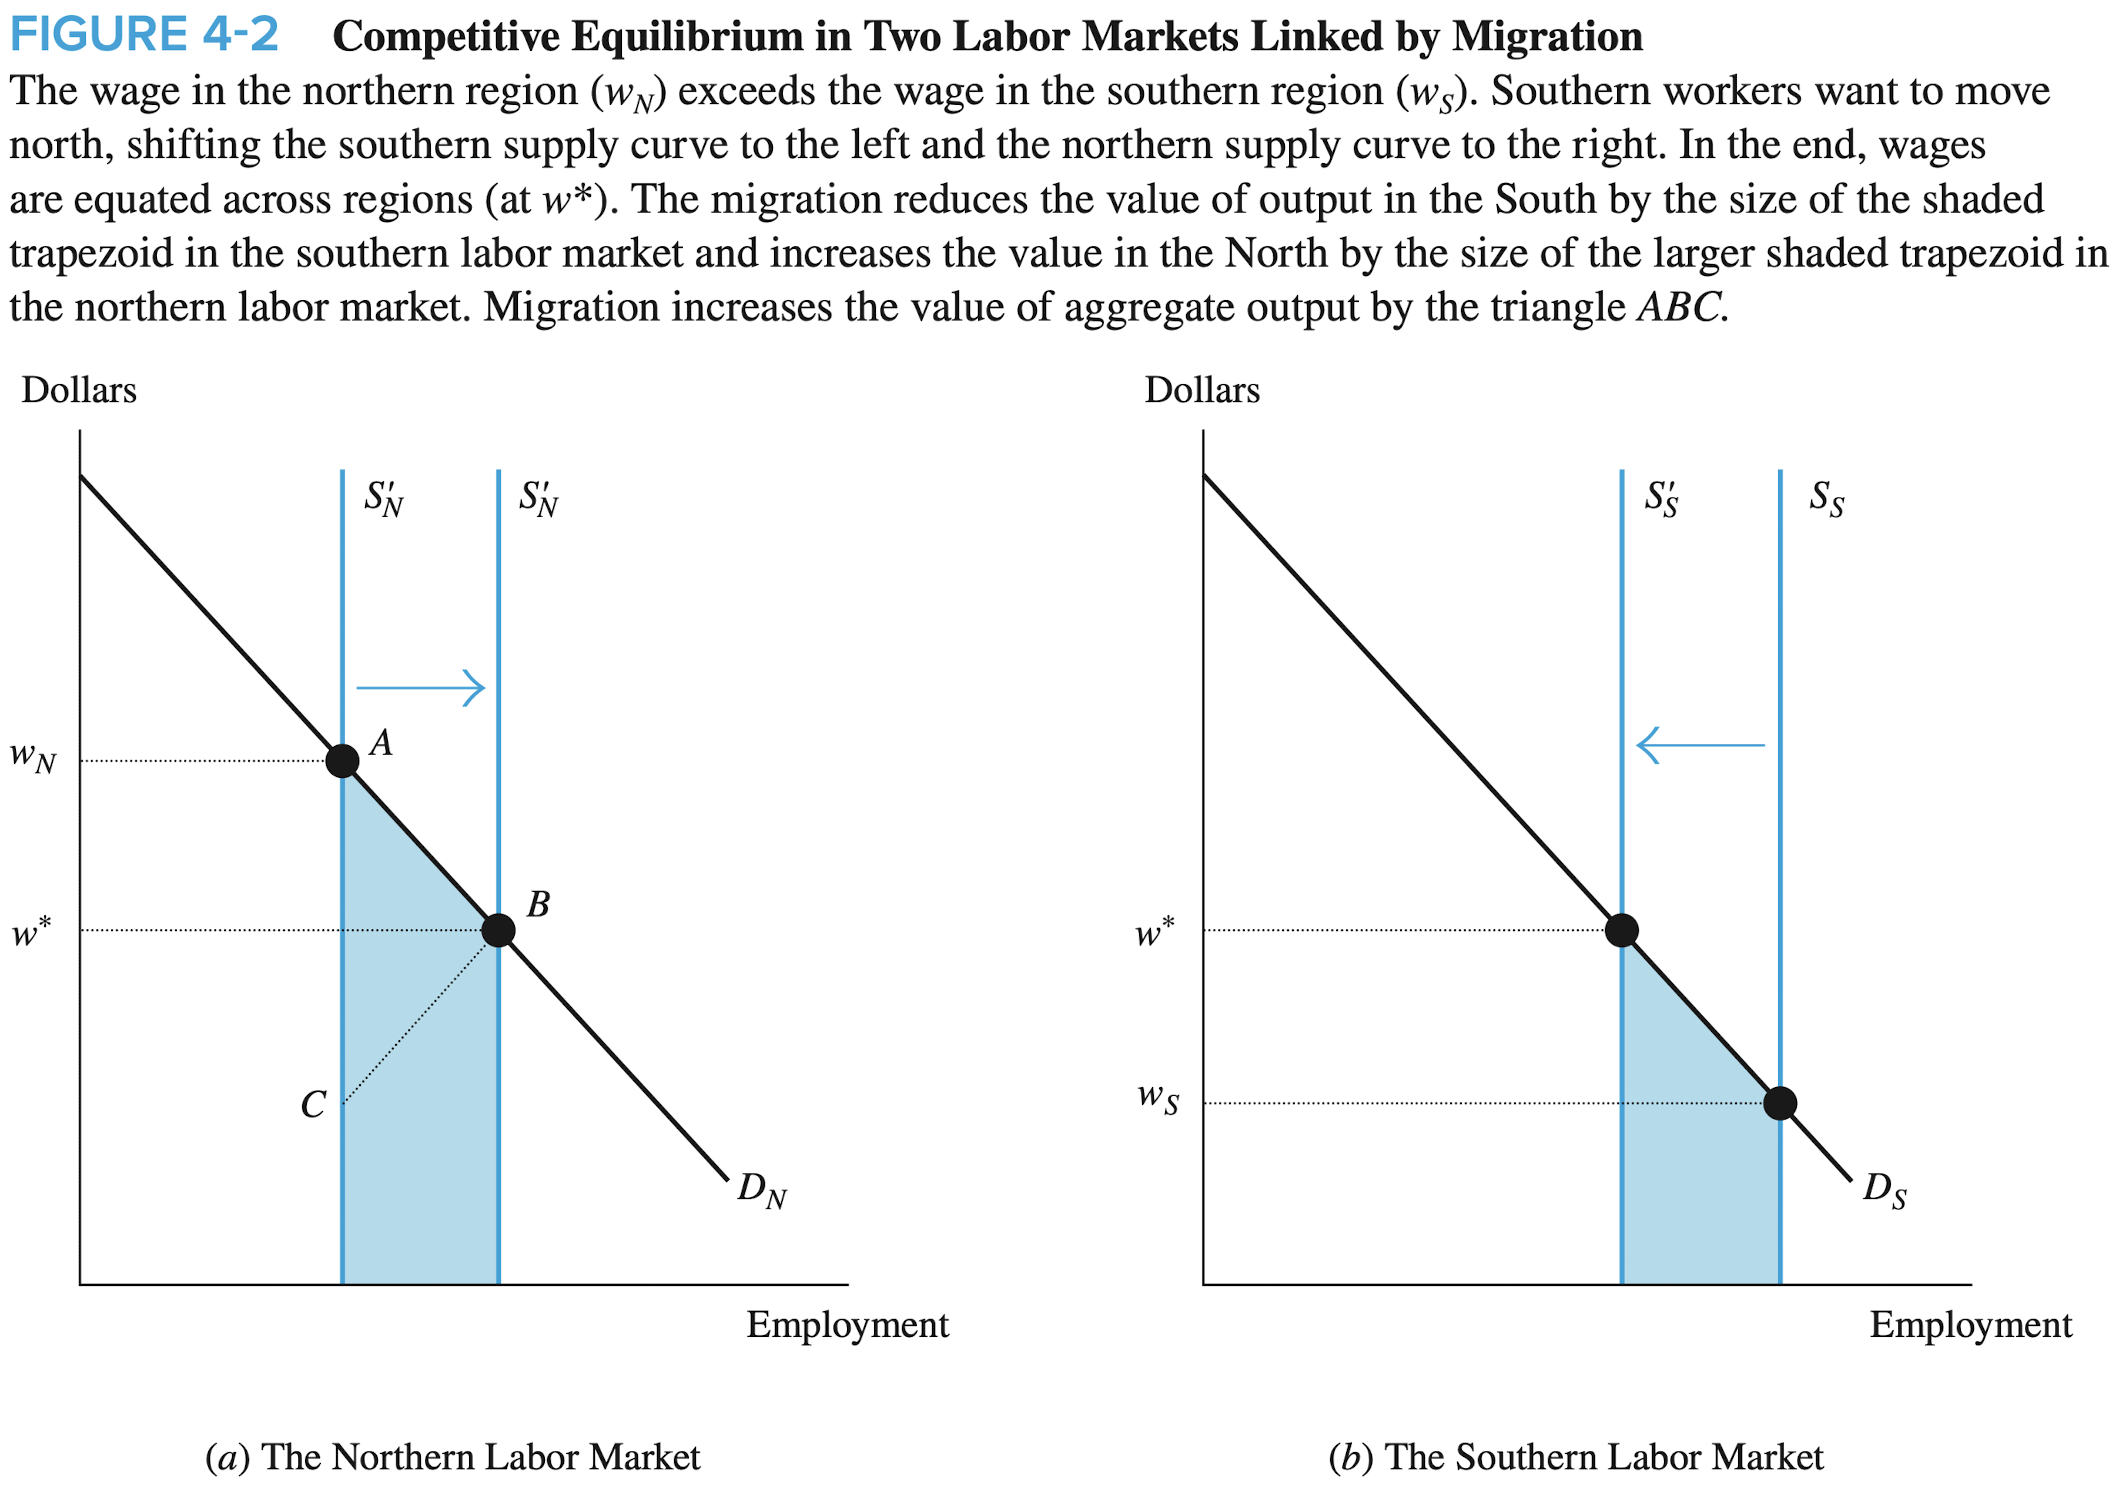
\includegraphics[width=0.95\textwidth]{../input/ch_4p2_multiple_markets.png}
    \caption{Equilibrium across Labor Markets}
    \label{fig:ch_4p2_multiple_markets}
\end{figure}
